\section{Bloc 1}

\begin{frame}{Com pensen els ordinadors/robots}
  \keyline{La informàtica no són només pantalles: és una manera d'entendre i transformar el món.}
  \begin{columns}[T,onlytextwidth]
    \column{0.49\textwidth}
    \centering
    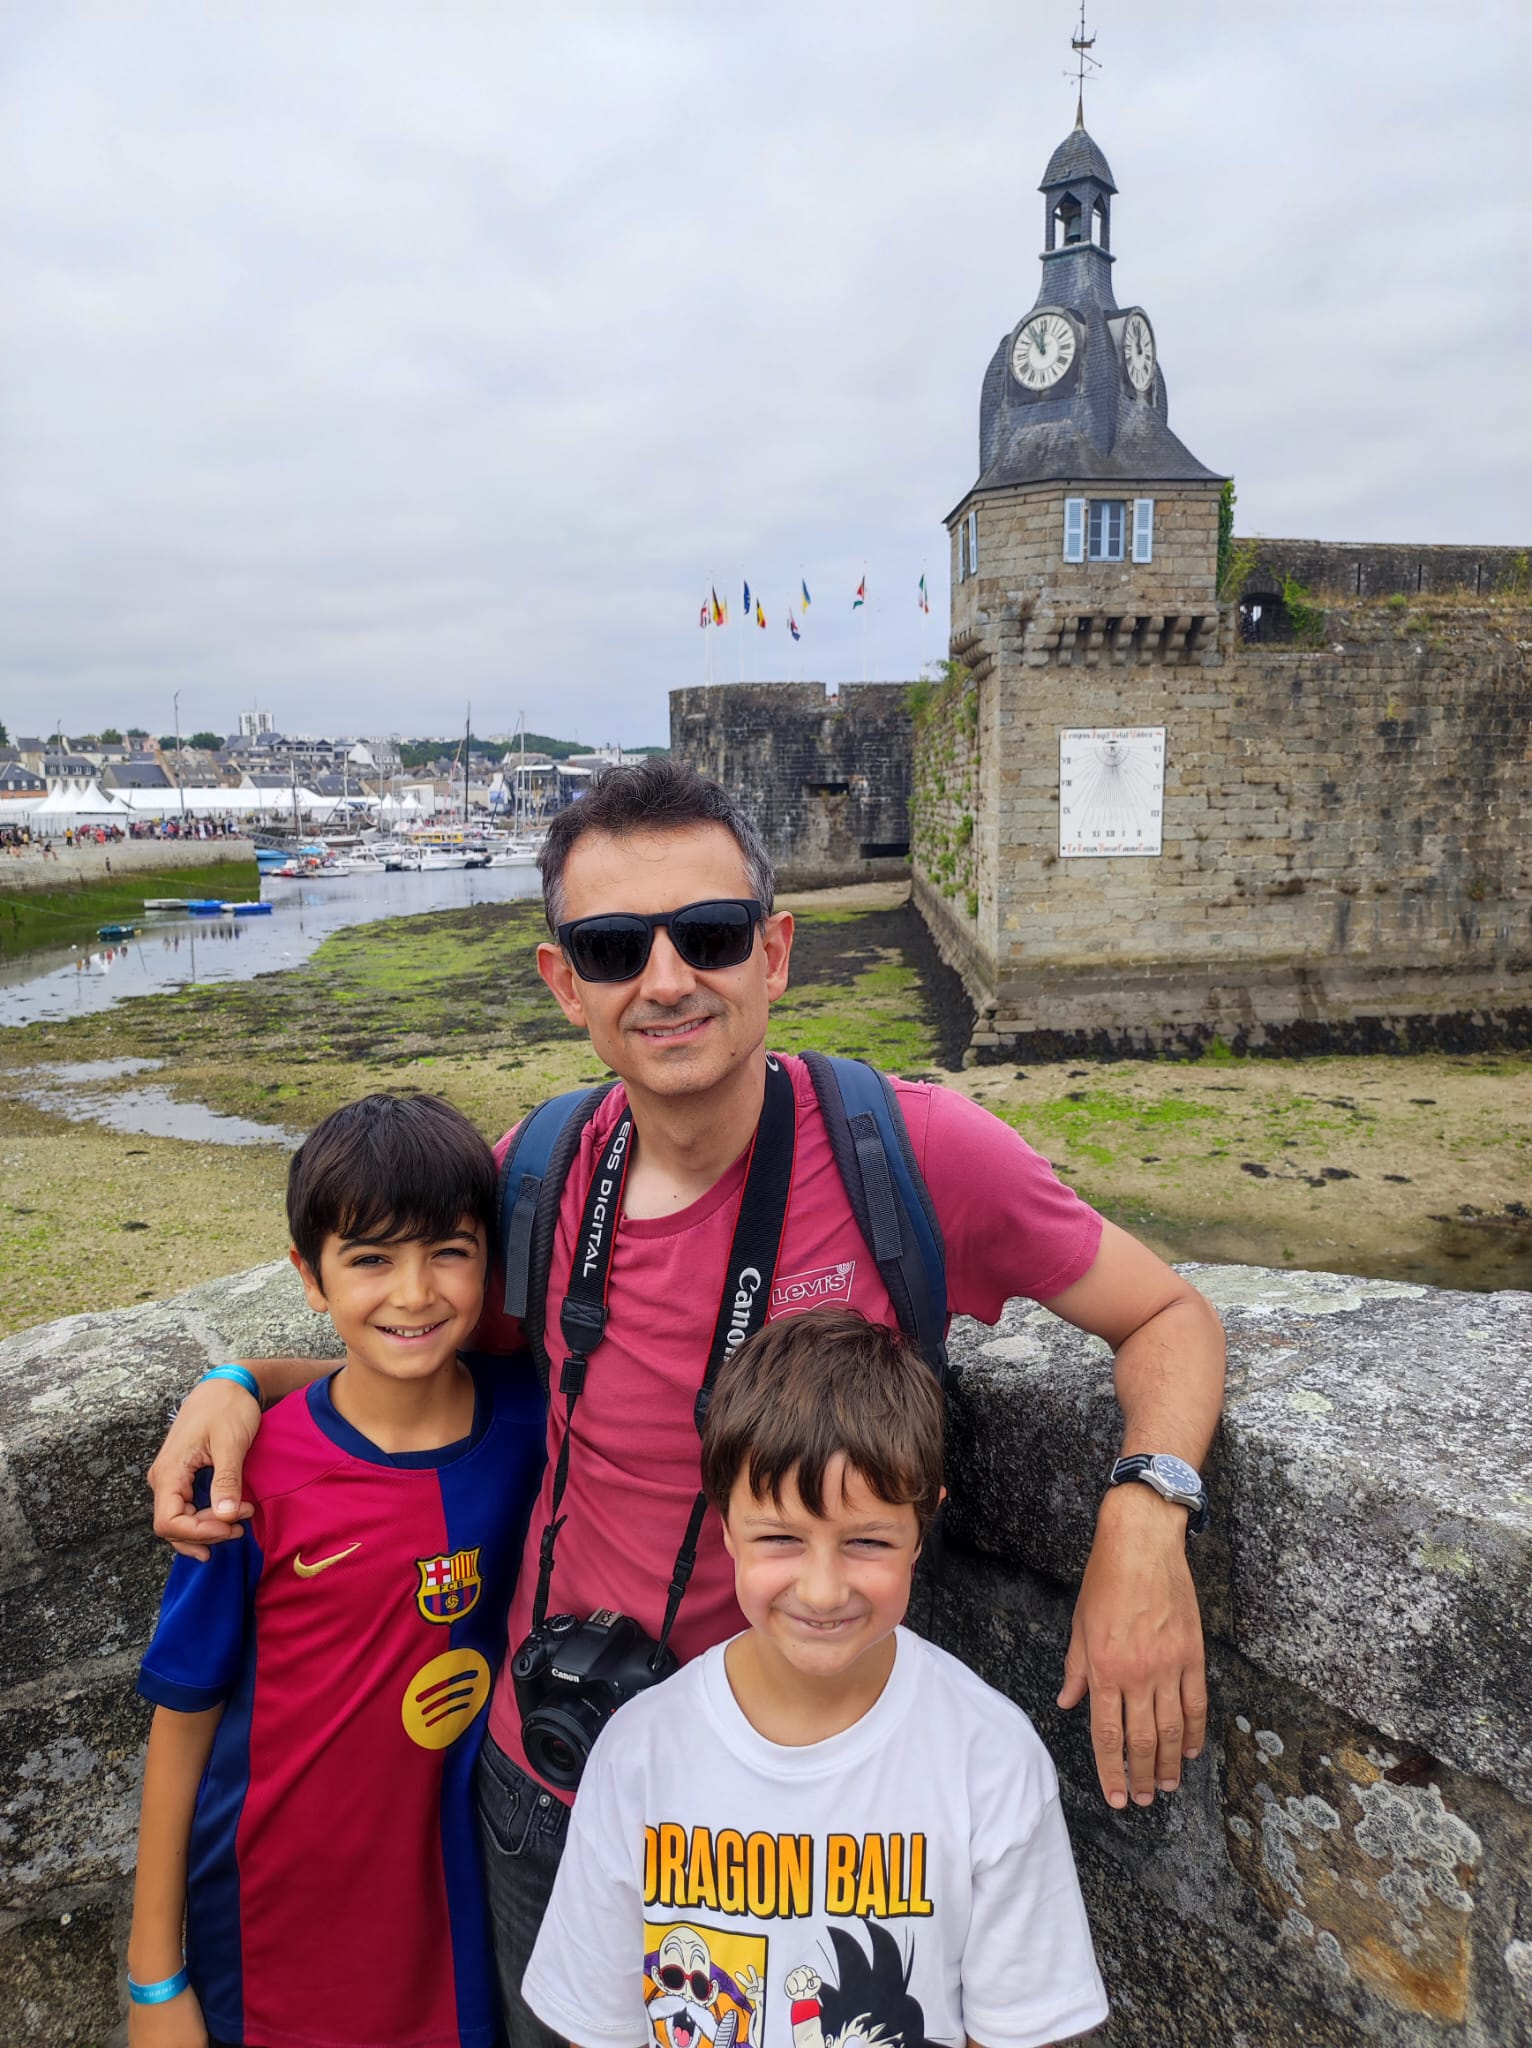
\includegraphics[width=\linewidth,height=0.53\textheight,keepaspectratio]{img/jo_i_nens.jpg}

    {\scriptsize jo i nens}
    \column{0.49\textwidth}
    \centering
    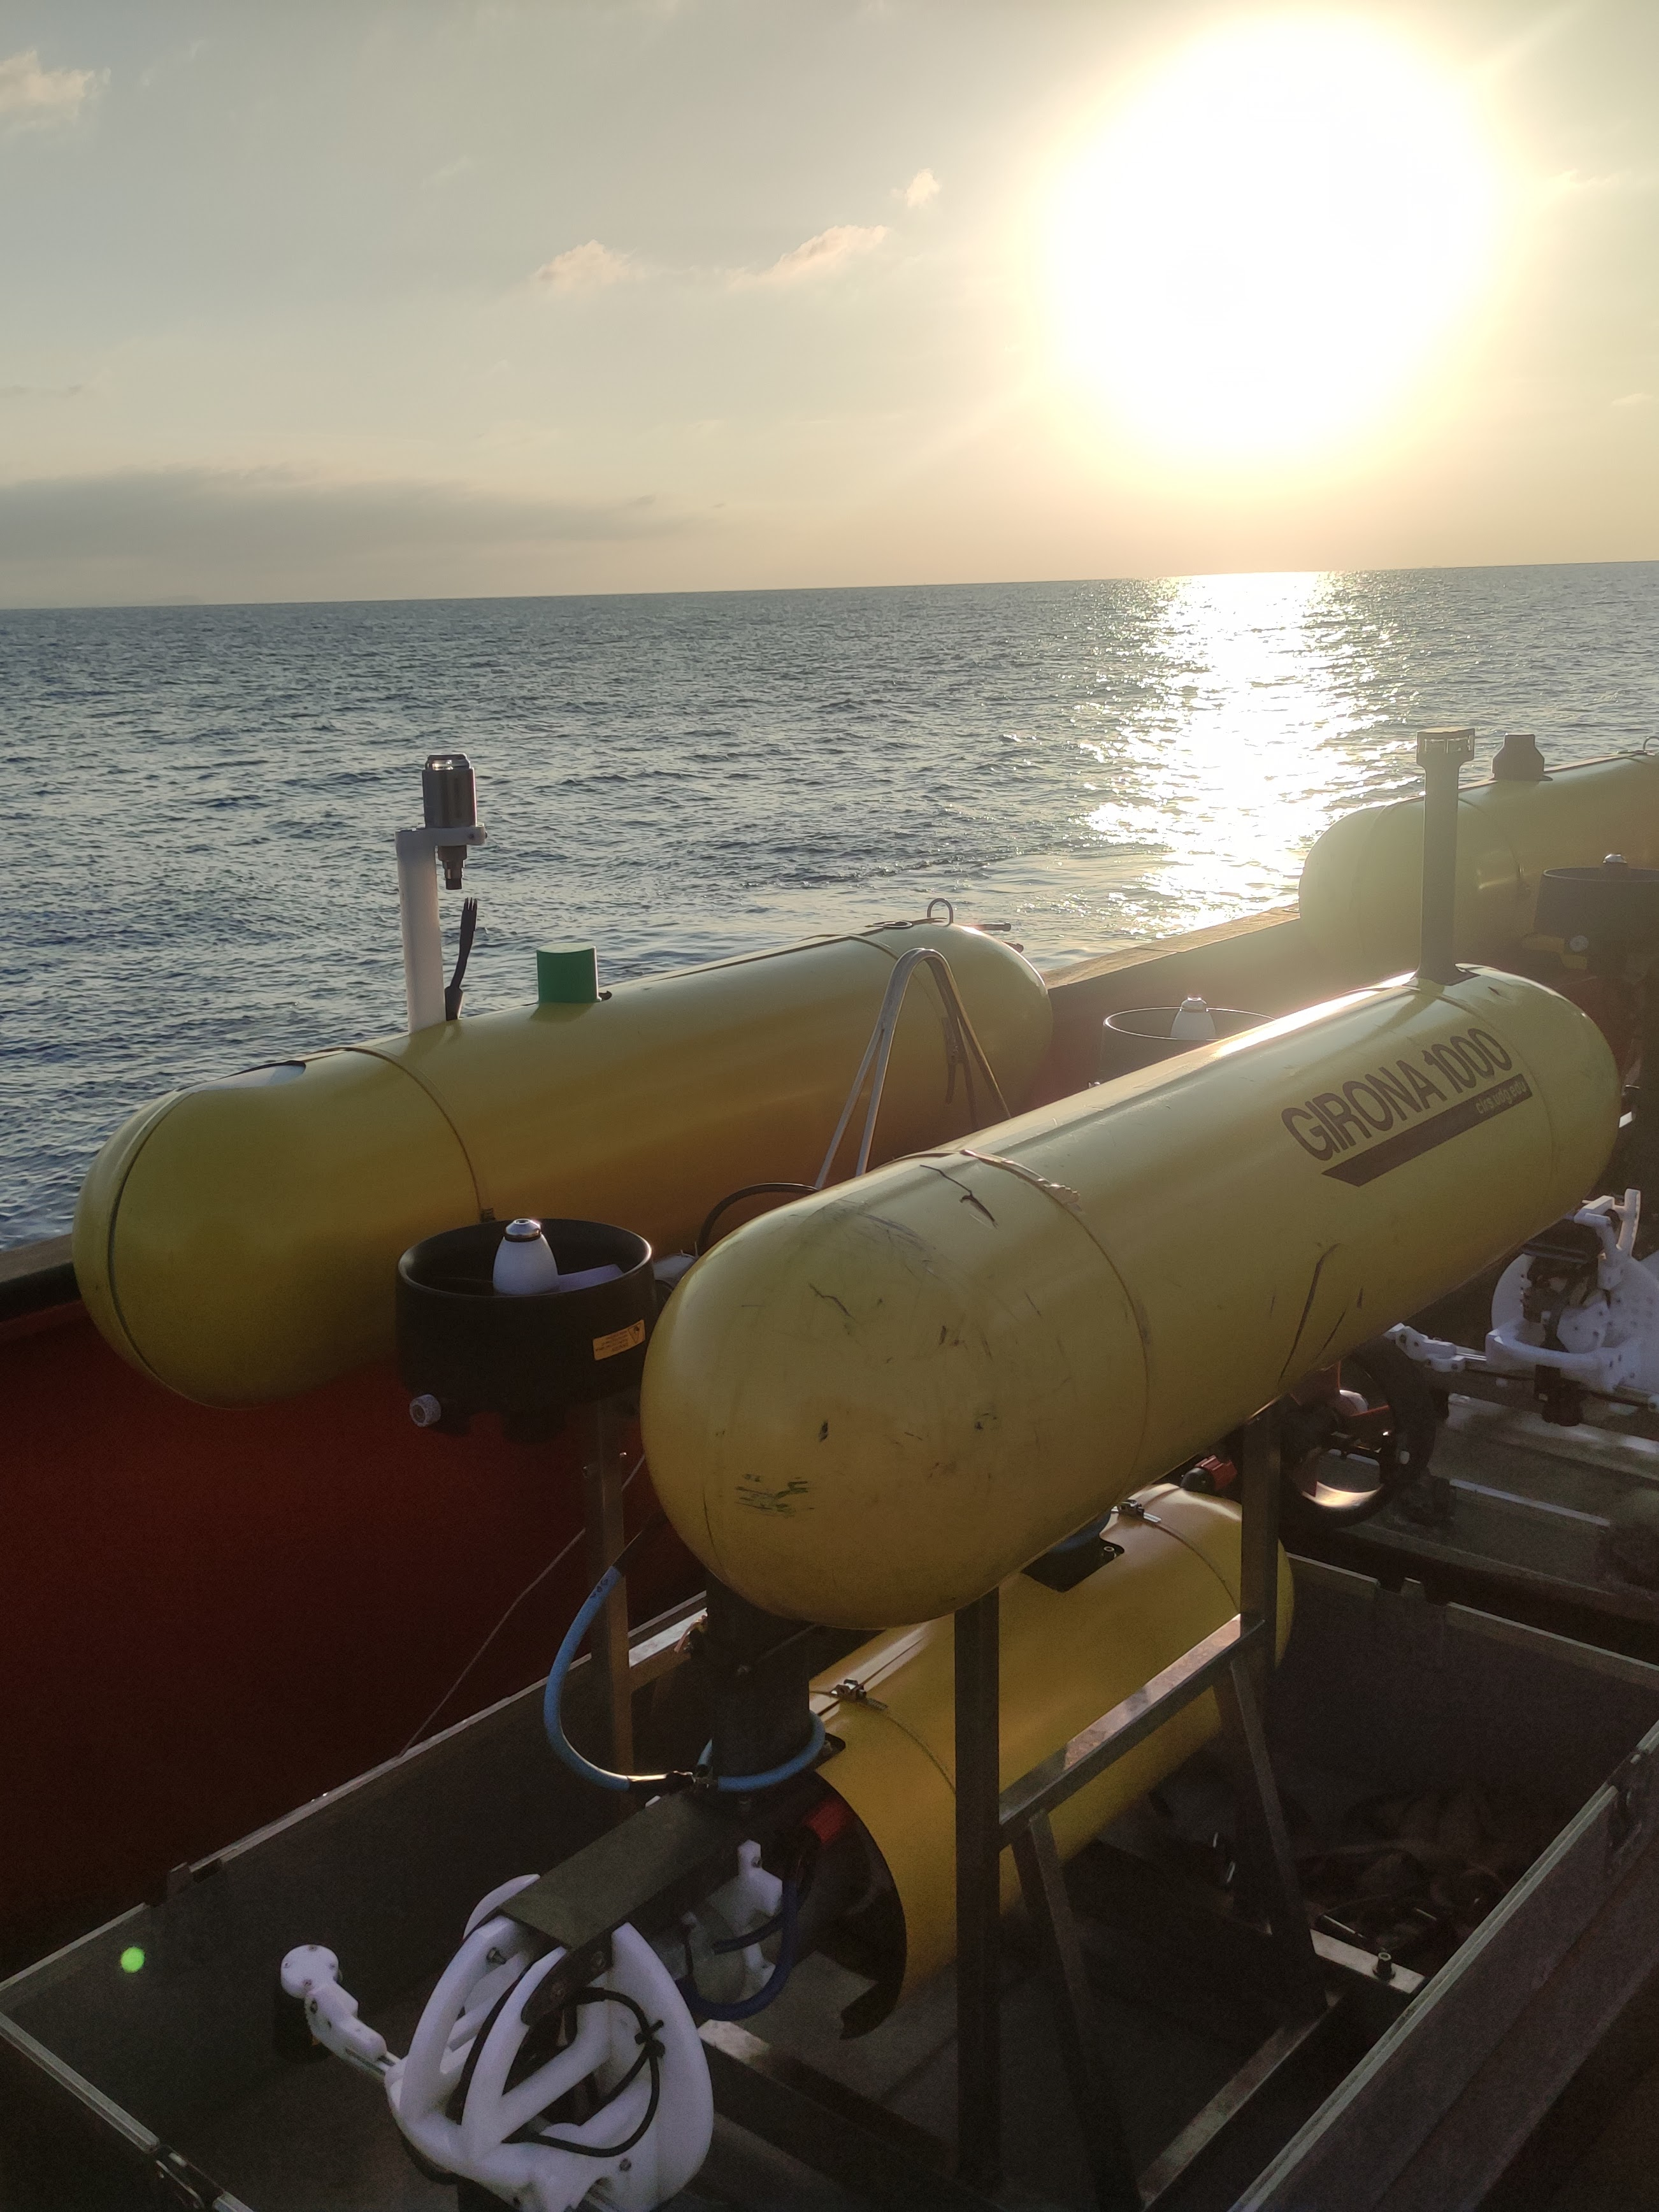
\includegraphics[width=\linewidth,height=0.53\textheight,keepaspectratio]{img/g1000_barco.jpg}

    {\scriptsize robot submarí Girona 1000}
  \end{columns}
  \twolinks{https://eia.udg.edu/ca/estudia/oferta-formativa/grau-en-enginyeria-informatica/}{https://www.youtube.com/@CIRSUdG}
\end{frame}

\begin{frame}{On apareix la ``informàtica'' al teu dia?}
  \keyline{Més llocs dels que sembla.}
  \centering
  \fbox{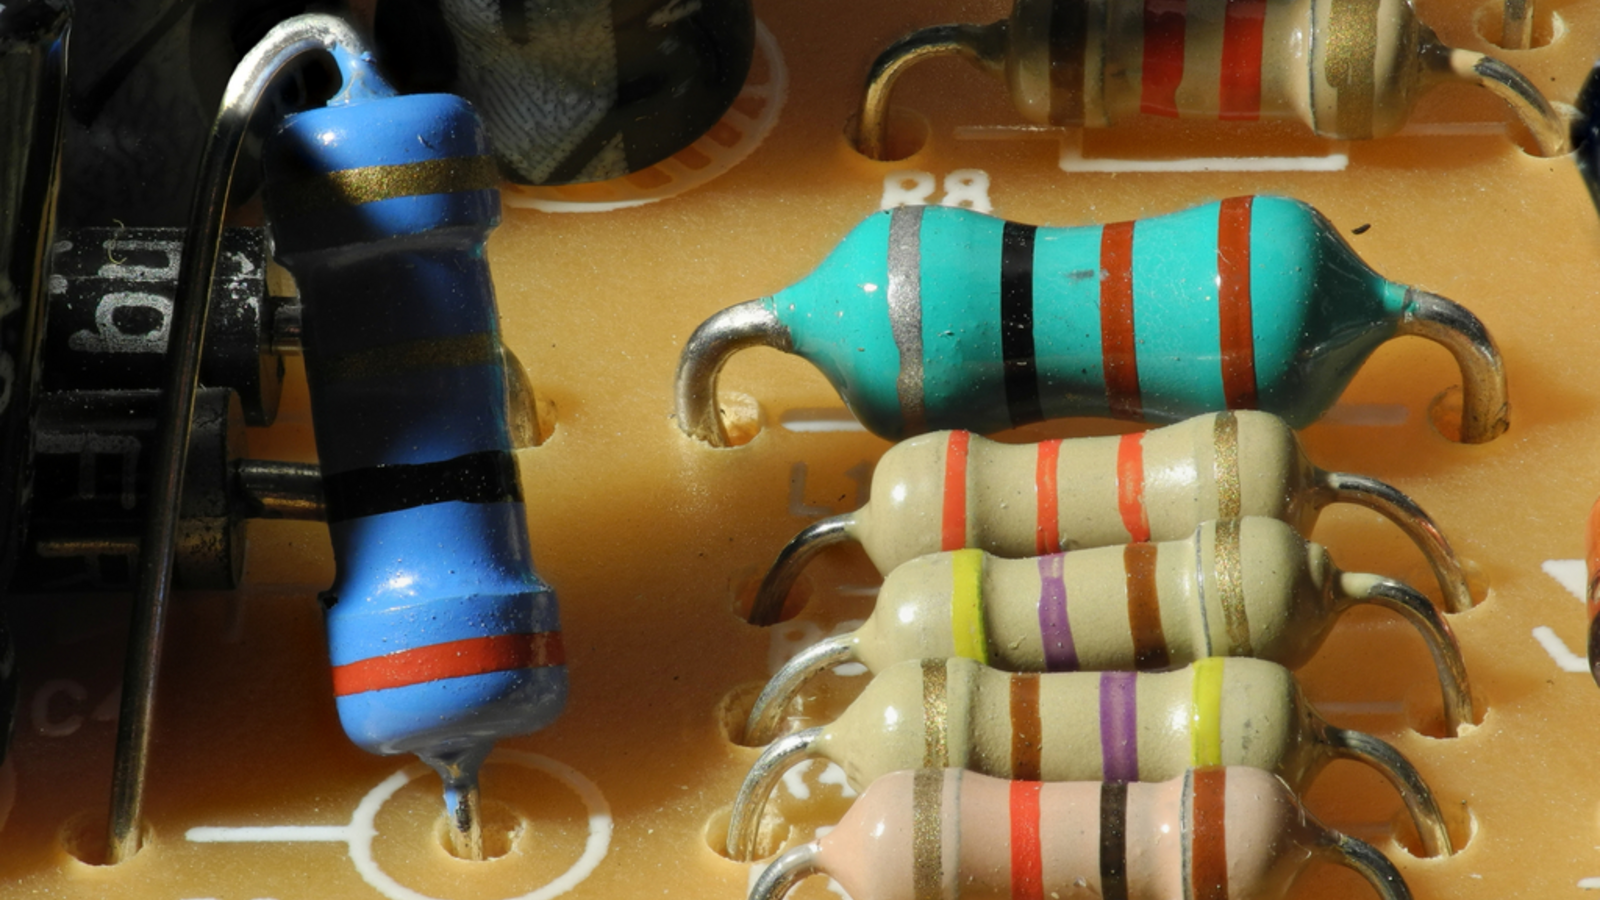
\includegraphics[width=0.9\linewidth,height=0.56\textheight]{img/slide02_dia.png}}

  {\scriptsize\itshape Font: Wikimedia Commons (\textit{Electronics devices (8386724198)}), Thomas Bresson, CC BY 2.0.}
  \slidelink{https://teachcomputing.org/curriculum/key-stage-2/computer-systems-and-networks}
\end{frame}

\begin{frame}{Com pensen els objectes: el ``cervell digital''}
  \keyline{Els objectes no pensen com nosaltres: executen instruccions.}
  \begin{columns}[T,onlytextwidth]
    \column{0.36\textwidth}
    \begin{itemize}
      \item Sensors
      \item Botons
      \item Pantalla
      \item Motor o actuador
    \end{itemize}
    \column{0.64\textwidth}
    \centering
    \fbox{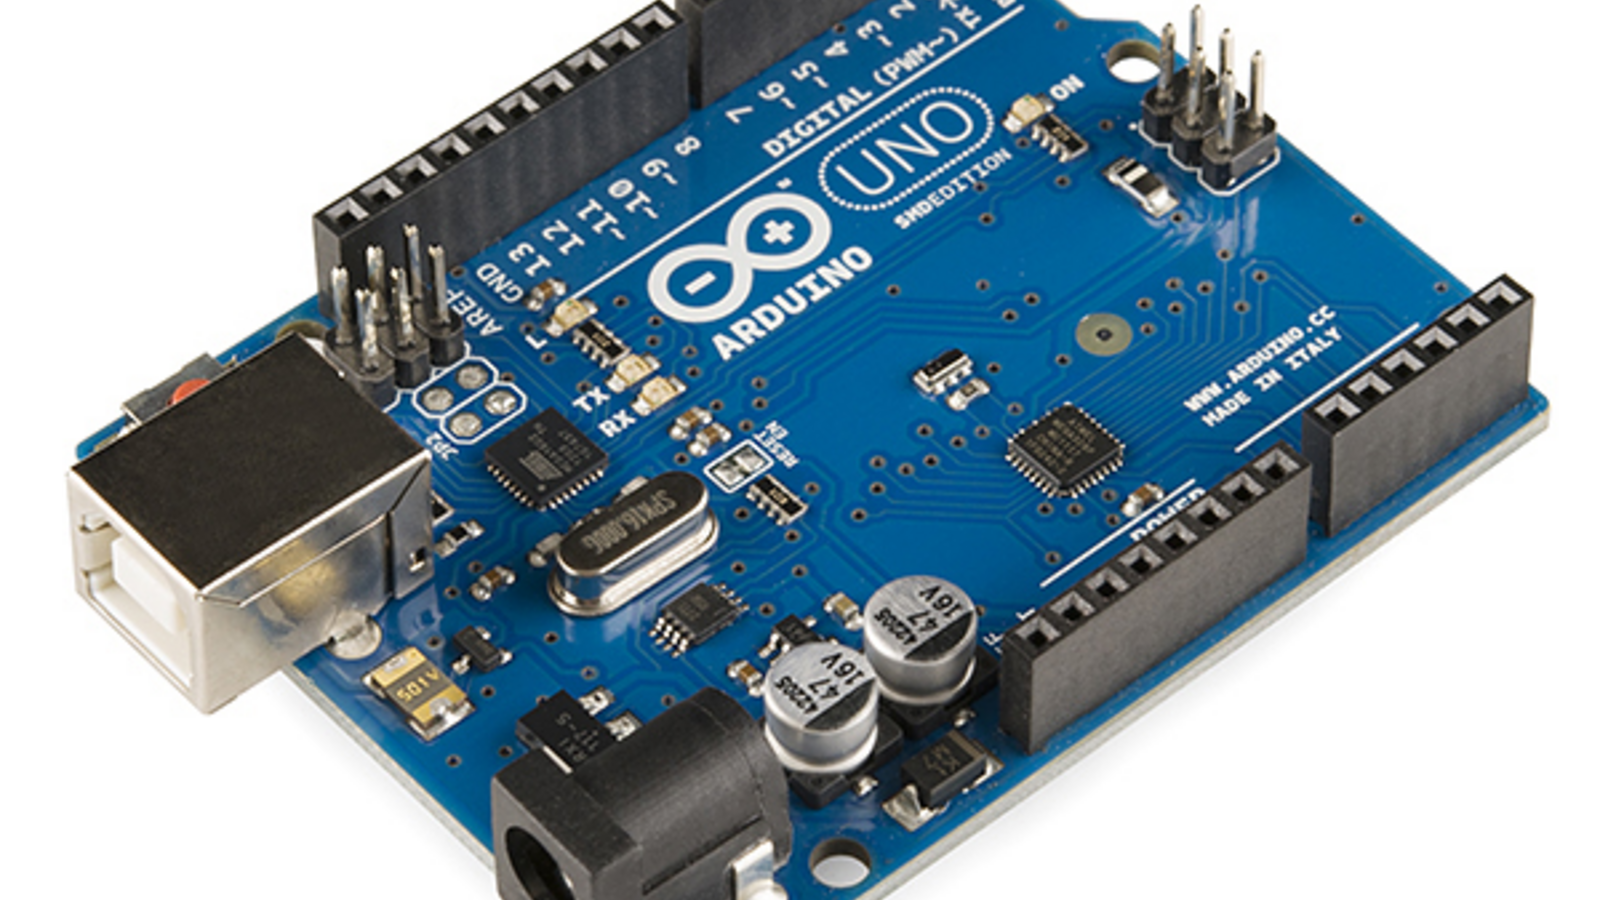
\includegraphics[width=\linewidth,height=0.52\textheight]{img/slide03_cervell_digital.png}}

    {\scriptsize\itshape Font: Wikimedia Commons (\textit{Arduino Uno - R3}), SparkFun Electronics, CC BY 2.0.}
  \end{columns}
  \twolinks{https://www.arduino.cc/}{https://www.ti.com/applications/industrial/factory-automation/embedded-processing.html}
\end{frame}

\begin{frame}{Com pensen els objectes: el ``cervell digital'' II}
  \keyline{Molts aparells reben dades, processen i responen.}
  \centering
  \fbox{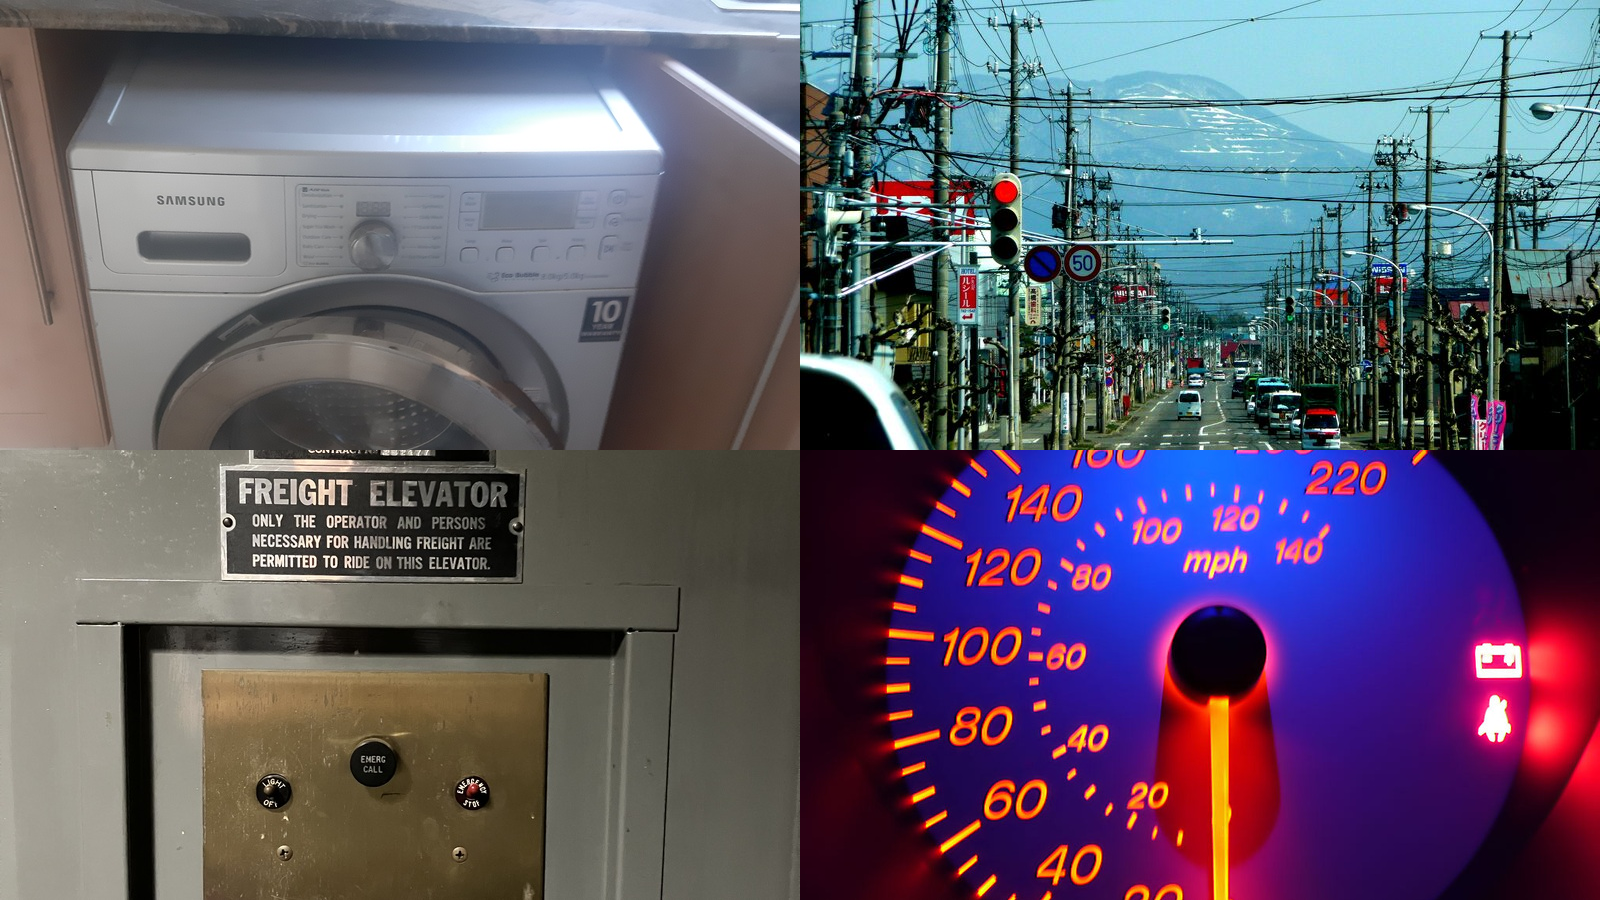
\includegraphics[width=0.93\linewidth,height=0.55\textheight]{img/slide04_entrades_proces_sortida.png}}

  {\scriptsize\itshape Collage amb 4 imatges de Wikimedia Commons: \textit{Front Load Washing Machine} (Fanti Salms, CC BY-SA 3.0), \textit{Traffic light in Aomori City; March 2008} (Herry Lawford, CC BY 2.0), \textit{Buttons of the elevator at Huron University college library} (Gogerr, CC BY 4.0), \textit{Car dashboard} (Mimiliz, CC BY-SA 3.0).}
  \slidelink{https://teachcomputing.org/curriculum/key-stage-2/computer-systems-and-networks}
\end{frame}

\begin{frame}{Els programes no només es troben dins d'objectes, també serveixen per crear-ne}
  \keyline{No només controla objectes: també ajuda a dissenyar, simular i decidir.}
  \centering
  \fbox{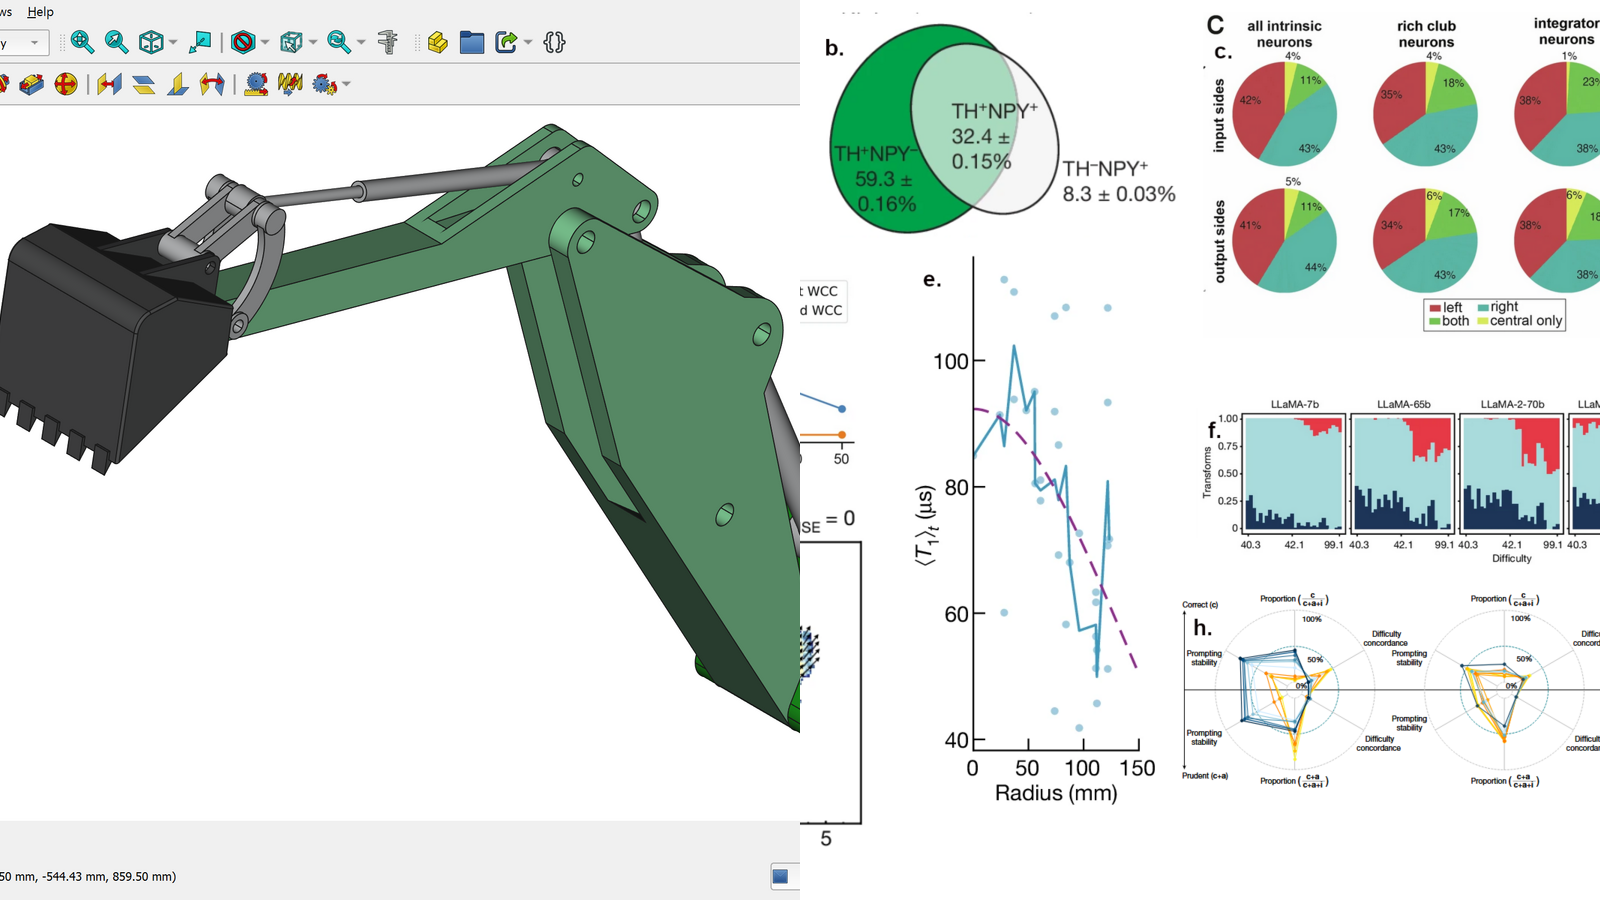
\includegraphics[width=0.93\linewidth,height=0.55\textheight]{img/slide05_programari_crea_mon.png}}

  {\scriptsize\itshape Collage amb 2 imatges de Wikimedia Commons: \textit{FreeCAD 1.0 Light Assembly Example} (Maxwxyz, CC BY 4.0) i \textit{Assortment scientific graphs} (RWhitwam, CC BY-SA 4.0).}
  \twolinks{https://www.iste.org/areas-of-focus/computational-thinking}{https://www.raspberrypi.org/teach/pedagogy/resources/computing-education-research}
\end{frame}

\begin{frame}{Programar és una supereina}
  \keyline{T'ajuda a automatitzar, provar idees i entendre millor la tecnologia.}
  \centering
  \fbox{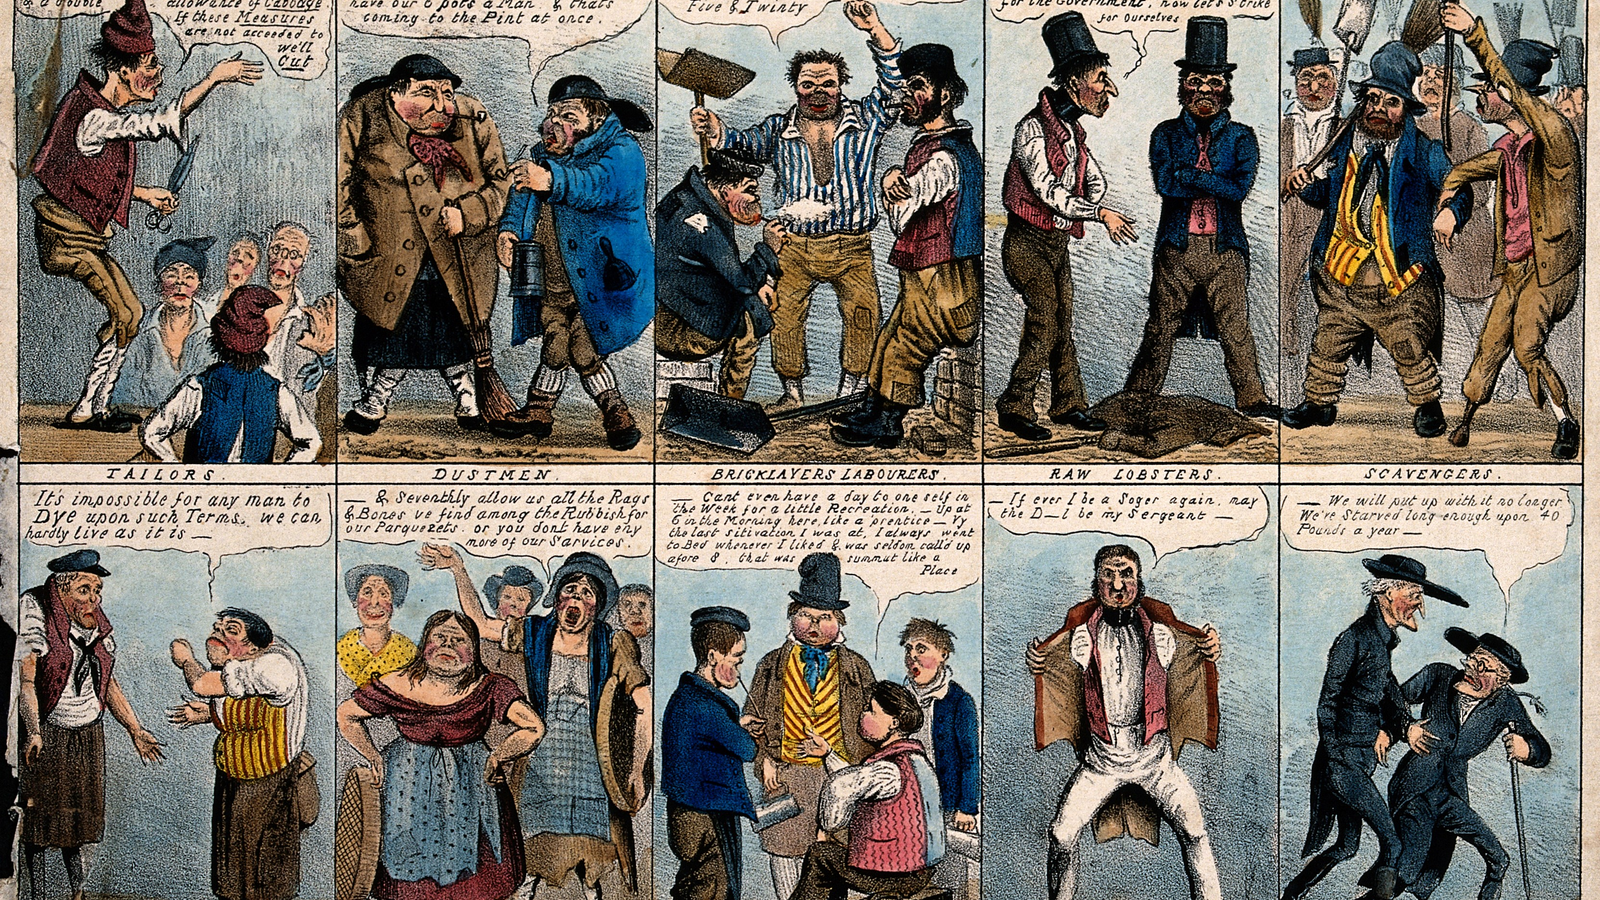
\includegraphics[width=0.93\linewidth,height=0.50\textheight]{img/slide06_supereina.png}}

  {\scriptsize\itshape Font: Wikimedia Commons (\textit{Groups of people with different trades and professions makin Wellcome V0039955}), Wellcome Collection, CC BY 4.0.}
  \twolinks{https://www.iste.org/areas-of-focus/computational-thinking}{https://k12cs.org/}
\end{frame}

\begin{frame}{El pensament computacional}
  \keyline{És una manera de resoldre problemes perquè una persona o una màquina els pugui seguir: descompondre, buscar patrons, abstraure i fer passos.}
  \begin{columns}[T,onlytextwidth]
    \column{0.42\textwidth}
    \begin{block}{Pensament computacional}
      una manera de resoldre problemes perquè una persona o una màquina els pugui seguir
    \end{block}
    \column{0.58\textwidth}
    \centering
    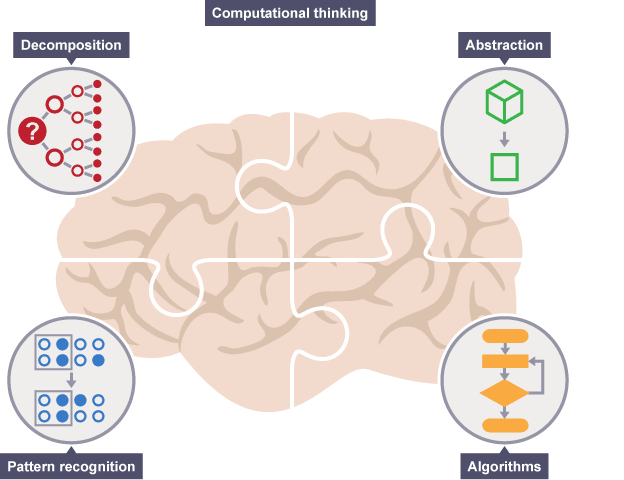
\includegraphics[width=\linewidth,height=0.55\textheight,keepaspectratio]{img/computational_thinking.png}
  \end{columns}
  \twolinks{https://www.iste.org/areas-of-focus/computational-thinking}{https://k12cs.org/computational-thinking/}
\end{frame}

\begin{frame}{Repte: com explicaries ``fer un entrepà'' a un robot?}
  \keyline{Si no ets precís, el robot s'equivoca.}
  \begin{columns}[T,onlytextwidth]
    \column{0.58\textwidth}
    \begin{enumerate}
      \item Agafa el pa
      \item Obre'l
      \item Posa el menjar
      \item Tanca'l
    \end{enumerate}
    \column{0.42\textwidth}
    \centering
    \begin{tikzpicture}[scale=0.9]
      \node[draw,rounded corners,fill=udgsand,minimum width=2.2cm,minimum height=1.4cm] at (0,0) {robot};
      \node[draw,rounded corners,fill=udgcoral!20,minimum width=2.2cm,minimum height=0.5cm] at (0,-1.3) {};
      \node[draw,rounded corners,fill=udgsand!50!white,minimum width=2.2cm,minimum height=0.5cm] at (0,-1.85) {};
      \draw[thick] (-0.6,0.7) -- (-1.2,1.2);
      \draw[thick] (0.6,0.7) -- (1.2,1.2);
    \end{tikzpicture}
  \end{columns}
  \twolinks{https://code.org/curriculum/course1/1/Teacher.pdf}{https://www.csunplugged.org/en/}
\end{frame}

\begin{frame}{Informàtica = treballar amb informació/dades}
  \keyline{Capturar, guardar, transformar i usar informació.}
  \centering
  \begin{tikzpicture}[node distance=1.5cm]
    \node[draw,rounded corners,fill=udgsand,minimum width=2.2cm,minimum height=1cm] (i) {informació};
    \node[draw,rounded corners,fill=udgblue!12,right=of i,minimum width=2.2cm,minimum height=1cm] (d) {dades};
    \node[draw,rounded corners,fill=udgteal!15,right=of d,minimum width=2.2cm,minimum height=1cm] (p) {programa};
    \node[draw,rounded corners,fill=udgcoral!18,right=of p,minimum width=2.2cm,minimum height=1cm] (r) {resultat};
    \draw[-{Latex[length=2mm]},thick] (i) -- (d);
    \draw[-{Latex[length=2mm]},thick] (d) -- (p);
    \draw[-{Latex[length=2mm]},thick] (p) -- (r);
  \end{tikzpicture}
  \slidelink{https://www.csfieldguide.org.nz/en/chapters/data-representation/}
\end{frame}

\begin{frame}{Què entenem per informació o dades?}
  \keyline{Tot això són dades.}
  \begin{center}
    \begin{tabular}{ccccc}
      text & imatges & so & números & sensors
    \end{tabular}
  \end{center}
  \vspace{0.6em}
  \begin{tikzpicture}[scale=0.95]
    \foreach \x/\label/\col in {
      0/HOLA/udgblue!12,
      2.3/IMG/udgteal!15,
      4.6/SO/udgcoral!18,
      6.9/42/udgsand,
      9.2/TEMP/udgblue!7
    }{
      \node[draw,rounded corners,fill=\col,minimum width=1.8cm,minimum height=1.2cm] at (\x,0) {\label};
    }
  \end{tikzpicture}
  \slidelink{https://www.csfieldguide.org.nz/en/chapters/data-representation/what-is-data-representation/}
\end{frame}

\begin{frame}{Els ordinadors representen totes les dades en dos estats; 1 i 0}
  \keyline{Per això parlem de 1 i 0.}
  \begin{columns}[T,onlytextwidth]
    \column{0.48\textwidth}
    \begin{block}{Metàfora}
      llum encesa / apagada\\
      interruptor sí / no
    \end{block}
    \column{0.52\textwidth}
    \centering
    \begin{tikzpicture}[scale=1]
      \draw[rounded corners,fill=udgsand] (0,0) rectangle (4,1.8);
      \fill[udgteal!70] (0.5,0.4) circle (0.4);
      \fill[white] (2.8,0.4) circle (0.4);
      \node at (0.5,1.25) {\Large 1};
      \node at (2.8,1.25) {\Large 0};
    \end{tikzpicture}
  \end{columns}
  \twolinks{https://www.csunplugged.org/en/topics/binary-numbers/}{https://www.csunplugged.org/en/at-home/binary-challenge/}
\end{frame}

\begin{frame}{Una lletra també es pot convertir en nombres}
  \keyline{Text $\rightarrow$ codi numèric $\rightarrow$ bits.}
  \centering
  \begin{tikzpicture}[node distance=1.4cm]
    \node[draw,rounded corners,fill=udgsand,minimum width=2cm,minimum height=1.3cm] (a) {\Huge A};
    \node[draw,rounded corners,fill=udgblue!12,right=of a,minimum width=2cm,minimum height=1.3cm] (b) {\Huge 65};
    \node[draw,rounded corners,fill=udgteal!15,right=of b,minimum width=3.2cm,minimum height=1.3cm] (c) {\Large 01000001};
    \draw[-{Latex[length=2mm]},thick] (a) -- (b);
    \draw[-{Latex[length=2mm]},thick] (b) -- (c);
  \end{tikzpicture}
  \twolinks{https://studio.code.org/courses/course4/units/1/lessons/18}{https://www.csfieldguide.org.nz/en/chapters/coding-compression-and-error-control/how-text-is-represented-in-binary/}
\end{frame}

\begin{frame}{Una imatge pot ser una graella}
  \keyline{Cada quadret és un píxel.}
  \begin{columns}[T,onlytextwidth]
    \column{0.55\textwidth}
    \centering
    \begin{tikzpicture}[scale=0.32]
      \foreach \x in {0,...,7} {
        \foreach \y in {0,...,7} {
          \draw[gray!60] (\x,\y) rectangle ++(1,1);
        }
      }
      \foreach \x/\y in {2/6,3/6,4/6,5/6,1/5,6/5,1/4,6/4,2/3,5/3,3/2,4/2} {
        \fill[udgcoral] (\x,\y) rectangle ++(1,1);
      }
    \end{tikzpicture}
    \column{0.45\textwidth}
    \begin{block}{Blanc o negre}
      cada píxel pot ser\\
      0 o 1
    \end{block}
  \end{columns}
  \twolinks{https://www.csunplugged.org/en/topics/image-representation/}{https://studio.code.org/s/course4/lessons/17/levels/1}
\end{frame}

\begin{frame}{En color, cada píxel guarda més informació}
  \keyline{Una barreja de vermell, verd i blau.}
  \begin{columns}[T,onlytextwidth]
    \column{0.55\textwidth}
    \centering
    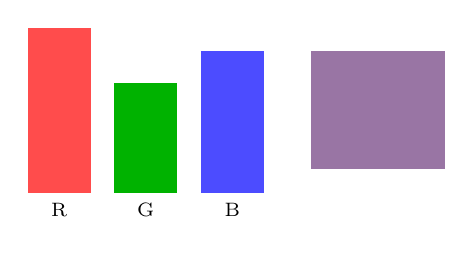
\begin{tikzpicture}[scale=1]
      \fill[red!70] (0,0) rectangle (0.8,2.1);
      \fill[green!70!black] (1.1,0) rectangle (1.9,1.4);
      \fill[blue!70] (2.2,0) rectangle (3,1.8);
      \fill[red!70!green!55!blue!65] (3.6,0.3) rectangle (5.3,1.8);
      \node[below] at (0.4,0) {\scriptsize R};
      \node[below] at (1.5,0) {\scriptsize G};
      \node[below] at (2.6,0) {\scriptsize B};
    \end{tikzpicture}
    \column{0.45\textwidth}
    \begin{block}{RGB}
      tres quantitats\\
      creen un color
    \end{block}
  \end{columns}
  \slidelink{https://www.csfieldguide.org.nz/en/chapters/data-representation/images-and-colours/}
\end{frame}

\begin{frame}{Un programa també és informació}
  \keyline{Les ordres i les dades es poden guardar en binari.}
  \centering
  \begin{tikzpicture}[node distance=2cm]
    \node[draw,rounded corners,fill=udgsand,minimum width=2.2cm,minimum height=1.2cm] (f) {foto};
    \node[draw,rounded corners,fill=udgblue!12,right=of f,minimum width=2.4cm,minimum height=1.2cm] (m) {memòria};
    \node[draw,rounded corners,fill=udgteal!15,below=1.1cm of f,minimum width=2.2cm,minimum height=1.2cm] (p) {programa};
    \draw[-{Latex[length=2mm]},thick] (f) -- (m);
    \draw[-{Latex[length=2mm]},thick] (p) -- (m);
    \node[below=0.3cm of m] {\scriptsize tot pot acabar representat com bits};
  \end{tikzpicture}
  \slidelink{https://www.csfieldguide.org.nz/en/chapters/data-representation/}
\end{frame}

\begin{frame}{Quatre peces bàsiques}
  \keyline{Fer passos, repetir, decidir i guardar valors.}
  \begin{center}
    \begin{tabular}{cccc}
      \fbox{seqüència} & \fbox{bucle} & \fbox{condició} & \fbox{variable}
    \end{tabular}
  \end{center}
  \vspace{0.8em}
  \begin{tikzpicture}[node distance=1.6cm]
    \node[draw,rounded corners,fill=udgsand,minimum width=1.8cm,minimum height=0.9cm] (a) {rebo};
    \node[draw,rounded corners,fill=udgblue!12,right=of a,minimum width=1.8cm,minimum height=0.9cm] (b) {faig};
    \node[draw,rounded corners,fill=udgteal!15,right=of b,minimum width=1.8cm,minimum height=0.9cm] (c) {decideixo};
    \node[draw,rounded corners,fill=udgcoral!18,right=of c,minimum width=1.8cm,minimum height=0.9cm] (d) {retorno};
    \draw[-{Latex[length=2mm]},thick] (a) -- (b);
    \draw[-{Latex[length=2mm]},thick] (b) -- (c);
    \draw[-{Latex[length=2mm]},thick] (c) -- (d);
  \end{tikzpicture}
  \twolinks{https://code.org/curriculum/docs/k-5/overview}{https://teachcomputing.org/curriculum/key-stage-2/programming-a}
\end{frame}

\begin{frame}{La mateixa idea es pot expressar de maneres diferents}
  \keyline{Canvia el format, no el repte.}
  \centering
  \begin{tikzpicture}[node distance=2.2cm]
    \node[draw,circle,fill=udgsand,minimum size=1.8cm] (r) {repte};
    \node[draw,rounded corners,fill=udgblue!12,above right=0.7cm and 1.5cm of r,minimum width=2cm,minimum height=0.9cm] (b) {blocs};
    \node[draw,rounded corners,fill=udgteal!15,right=of r,minimum width=2cm,minimum height=0.9cm] (t) {text};
    \node[draw,rounded corners,fill=udgcoral!18,below right=0.7cm and 1.5cm of r,minimum width=2cm,minimum height=0.9cm] (a) {aprendre};
    \draw[-{Latex[length=2mm]},thick] (r) -- (b);
    \draw[-{Latex[length=2mm]},thick] (r) -- (t);
    \draw[-{Latex[length=2mm]},thick] (r) -- (a);
  \end{tikzpicture}
  \twolinks{https://scratch.mit.edu/}{https://experience-ai.org/en/units/machine-learning-and-pattern-recognition/}
\end{frame}

\begin{frame}{Scratch: programar encaixant peces}
  \keyline{És visual i molt bona per començar.}
  \begin{columns}[T,onlytextwidth]
    \column{0.56\textwidth}
    \centering
    \begin{tikzpicture}[scale=0.9]
      \node[draw,rounded corners,fill=udgblue!15,minimum width=4.6cm,minimum height=0.75cm] at (0,2.3) {quan es premi bandera verda};
      \node[draw,rounded corners,fill=udgteal!18,minimum width=3.2cm,minimum height=0.75cm] at (-0.35,1.3) {repeteix 4 vegades};
      \node[draw,rounded corners,fill=udgsand,minimum width=2.4cm,minimum height=0.75cm] at (-0.65,0.35) {mou 10 passos};
      \node[draw,rounded corners,fill=udgcoral!18,minimum width=2.8cm,minimum height=0.75cm] at (-0.45,-0.6) {si toca vora...};
    \end{tikzpicture}
    \column{0.44\textwidth}
    \begin{itemize}
      \item sense sintaxi difícil
      \item idees clares
      \item jocs i històries
    \end{itemize}
  \end{columns}
  \twolinks{https://scratch.mit.edu/about}{https://scratch.mit.edu/ideas}
\end{frame}

\begin{frame}{El mateix programa, escrit amb paraules}
  \keyline{Python o pseudocodi expressen les mateixes idees.}
  \begin{columns}[T,onlytextwidth]
    \column{0.48\textwidth}
    \begin{block}{Blocs}
      repeteix\\
      mou\\
      si...
    \end{block}
    \column{0.52\textwidth}
    \begin{block}{Text}
\texttt{for i in range(4):}\\
\texttt{\ \ move(10)}\\
\texttt{\ \ if edge(): turn()}
    \end{block}
  \end{columns}
  \slidelink{https://www.raspberrypi.org/learn/pathways/scratch-to-python/}
\end{frame}

\begin{frame}{Per què tanta gent programa amb text?}
  \keyline{És compacte, flexible i molt potent.}
  \begin{columns}[T,onlytextwidth]
    \column{0.58\textwidth}
    \begin{itemize}
      \item projectes grans
      \item fitxers i versions
      \item més control
    \end{itemize}
    \column{0.42\textwidth}
    \centering
    \begin{tikzpicture}[scale=0.95]
      \draw[fill=udgsand,rounded corners] (0,0) rectangle (3.8,2.5);
      \foreach \y in {2.0,1.5,1.0,0.5} {
        \draw[udggray,line width=1pt] (0.5,\y) -- (3.2,\y);
      }
      \draw[udgcoral,line width=1.3pt] (1.4,1.5) circle (0.45);
    \end{tikzpicture}
  \end{columns}
  \twolinks{https://scratch.mit.edu/about}{https://www.raspberrypi.org/learn/pathways/scratch-to-python/}
\end{frame}

\begin{frame}{Manera 1: escriure les regles}
  \keyline{La persona decideix els passos.}
  \centering
  \begin{tikzpicture}[node distance=1.8cm]
    \node[draw,rounded corners,fill=udgsand,minimum width=1.8cm,minimum height=1cm] (h) {humà};
    \node[draw,rounded corners,fill=udgblue!12,right=of h,minimum width=2.4cm,minimum height=1cm] (r) {regles};
    \node[draw,rounded corners,fill=udgteal!15,right=of r,minimum width=2.2cm,minimum height=1cm] (o) {ordinador};
    \node[draw,rounded corners,fill=udgcoral!18,right=of o,minimum width=2.2cm,minimum height=1cm] (res) {resultat};
    \draw[-{Latex[length=2mm]},thick] (h) -- (r);
    \draw[-{Latex[length=2mm]},thick] (r) -- (o);
    \draw[-{Latex[length=2mm]},thick] (o) -- (res);
  \end{tikzpicture}
  \slidelink{https://experience-ai.org/en/units/introduction-to-ai/what-is-ai/}
\end{frame}

\begin{frame}{Manera 2: ensenyar amb molts exemples}
  \keyline{Li mostrem dades i etiquetes.}
  \begin{columns}[T,onlytextwidth]
    \column{0.5\textwidth}
    \begin{itemize}
      \item peix / plàstic
      \item gat / gos
      \item bo / dolent
    \end{itemize}
    \column{0.5\textwidth}
    \centering
    \begin{tikzpicture}[scale=0.9]
      \node[draw,rounded corners,fill=udgsand,minimum width=1.7cm,minimum height=1cm] at (0,1.4) {foto 1};
      \node[draw,rounded corners,fill=udgsand,minimum width=1.7cm,minimum height=1cm] at (0,0) {foto 2};
      \node[draw,rounded corners,fill=udgblue!12,minimum width=2.2cm,minimum height=2.6cm] at (3,0.7) {model};
      \draw[-{Latex[length=2mm]},thick] (0.9,1.4) -- (1.8,1.0);
      \draw[-{Latex[length=2mm]},thick] (0.9,0) -- (1.8,0.4);
    \end{tikzpicture}
  \end{columns}
  \threelinks{https://teachablemachine.withgoogle.com/}{https://dayofai.org/}{https://quickdraw.withgoogle.com/}
\end{frame}

\begin{frame}{Manera 3: provar moltes vegades i rebre punts}
  \keyline{Si ho fa bé, recompensa; si no, torna a provar.}
  \begin{columns}[T,onlytextwidth]
    \column{0.55\textwidth}
    \centering
    \begin{tikzpicture}[scale=0.95]
      \node[draw,circle,fill=udgsand,minimum size=1cm] (a) at (0,0) {1};
      \node[draw,circle,fill=udgsand,minimum size=1cm] (b) at (2,1.2) {2};
      \node[draw,circle,fill=udgsand,minimum size=1cm] (c) at (2,-1.2) {3};
      \node[draw,star,star points=5,fill=yellow!60,minimum size=0.9cm] (g) at (4.2,0) {};
      \draw[-{Latex[length=2mm]},thick] (a) -- (b);
      \draw[-{Latex[length=2mm]},thick] (a) -- (c);
      \draw[-{Latex[length=2mm]},thick] (b) -- (g);
      \draw[-{Latex[length=2mm]},thick] (c) -- (g);
    \end{tikzpicture}
    \column{0.45\textwidth}
    \begin{block}{Com un videojoc}
      prova\\
      s'equivoca\\
      millora
    \end{block}
  \end{columns}
  \twolinks{https://deepmind.google/discover/blog/alphazero-shedding-new-light-on-chess-shogi-and-go/}{https://developer.nvidia.com/blog/reinforcement-learning-for-robotics/}
\end{frame}

\begin{frame}{Avui també podem treballar parlant amb una IA}
  \keyline{Un prompt pot ajudar, però no substitueix entendre el problema.}
  \centering
  \begin{tikzpicture}[node distance=1.4cm]
    \node[draw,rounded corners,fill=udgsand,minimum width=1.8cm,minimum height=0.9cm] (p) {persona};
    \node[draw,rounded corners,fill=udgblue!12,right=of p,minimum width=1.8cm,minimum height=0.9cm] (pr) {prompt};
    \node[draw,rounded corners,fill=udgteal!15,right=of pr,minimum width=1.8cm,minimum height=0.9cm] (ia) {IA};
    \node[draw,rounded corners,fill=udgcoral!18,right=of ia,minimum width=2.2cm,minimum height=0.9cm] (es) {esborrany};
    \node[draw,rounded corners,fill=udgsand,below=1.1cm of es,minimum width=2.7cm,minimum height=0.9cm] (cv) {comprovació humana};
    \draw[-{Latex[length=2mm]},thick] (p) -- (pr);
    \draw[-{Latex[length=2mm]},thick] (pr) -- (ia);
    \draw[-{Latex[length=2mm]},thick] (ia) -- (es);
    \draw[-{Latex[length=2mm]},thick] (es) -- (cv);
  \end{tikzpicture}
  \threelinks{https://code.org/artificial-intelligence}{https://dayofai.org/}{https://www.unesco.org/en/articles/guidance-generative-ai-education-and-research}
\end{frame}

\begin{frame}{La IA és potent, però no és màgia}
  \keyline{Aprèn de dades, pot fallar i cal comprovar-la.}
  \begin{columns}[T,onlytextwidth]
    \column{0.33\textwidth}
    \begin{block}{ajuda}
      ràpida
    \end{block}
    \column{0.33\textwidth}
    \begin{alertblock}{error}
      es pot equivocar
    \end{alertblock}
    \column{0.33\textwidth}
    \begin{block}{comprova}
      responsabilitat humana
    \end{block}
  \end{columns}
  \vspace{0.8em}
  \centering
  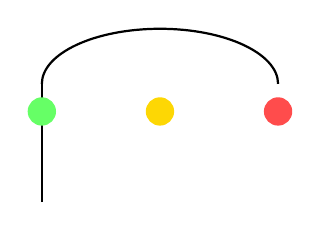
\begin{tikzpicture}
    \draw[thick] (0,0) -- (0,1.5);
    \draw[thick] (0,1.5) arc (180:0:1.5 and 0.7);
    \fill[green!60] (0,1.15) circle (0.18);
    \fill[yellow!75!orange] (1.5,1.15) circle (0.18);
    \fill[red!70] (3,1.15) circle (0.18);
  \end{tikzpicture}
  \twolinks{https://dayofai.org/}{https://www.unesco.org/en/articles/guidance-generative-ai-education-and-research}
\end{frame}
